\documentclass{ua_wgs_base}

\hypersetup{pdftitle={Remote Identification and Tracking for Unmanned Aircraft Systems},
 pdfauthor={UTM Working Group},
 pdfsubject={Remote Identification and Tracking for Unmanned Aircraft Systems},
 pdfkeywords={Unmanned Aircraft Systems, Remote ID, Tracking},
 pdfpagelayout=OneColumn, pdfnewwindow=true, pdfstartview=XYZ, plainpages=false}

\begin{document}

\title{Remote Identification and Tracking for Unmanned Aircraft Systems}

\author{UTM Working Group}

\maketitle
\cleardoublepage{}
\begin{abstract}
This report describes a consensus based Remote Identification and
Tracking Standard for Unmanned Aircraft Systems in India in the context
of ASTM \nomenclature{ASTM}{ASTM International, formerly American Society for Testing and Materials; an international standards organization that develops and publishes consensus technical standards for a wide range of materials, products, systems, and services.}
Remote ID Specification and the NPNT \nomenclature{NPNT}{No Permission No Take-off; a cryptographically secure process for programming and flying UASs in India}Regulation
in India. It focuses on the way forward for stakeholders to enable
remote identification of their systems by law enforcement and other
third parties.

Keywords: Unmanned Aviation, Unmanned Aircraft Systems, Drones, Identification,
Risk Assessment, Law Enforcement, Counter-UAS

\tableofcontents{}
\end{abstract}

\chapter*{Working Group\label{sec:wg}}

\addcontentsline{toc}{section}{\nameref{sec:wg}}

This working group meets almost weekly to discuss the roles, responsibilities
and activities to be performed by a Unmanned Traffic Management Service
Provider (UTM-SP)\nomenclature{DSP}{DigitalSky Service Provider; used interchangeably with UTM-SP}\nomenclature{UTM}{Unmanned Traffic Management; an activity similar to Air Traffic Management for manned flights}\nomenclature{UTM-SP}{UTM Service Provider; an organisation providing UTM services, including but not limited to Remote Identification and Tracking of UASs; used interchangeably with DSP}
in the context of Indian drone industry. It also aims to document
the ways in which a UTM-SP interacts with other stakeholders in the
industry, namely, manufacturers, operators, pilots, UFII, and so forth.
The documentation would be put through as recommendations to DGCA\nomenclature{DGCA}{Directorate General of Civil Aviation, MoCA},
MoCA,\nomenclature{MoCA}{Ministry of Civil Aviation, Government of India}
and other relevant parties as it matures.

\begin{figure}[tbh]
\begin{centering}
\begin{center}
\small\tt
\hfil 
\xymatrix{ & \txt{DFI} \ar[dr] & \txt{MoCA} \ar[d] & \cdots \ar[dl] & \\ 
& & \txt{UA Society} \ar[d] & & \\
& & \txt{Steering \\Committee} \ar[dl] \ar[dr] & & \\
& \txt{Working Groups} \ar[dl] \ar[d] & & \txt{Research Groups} \ar[dl] \ar[d] \ar[dr] & \\
\cdots \ar[r] & *+[F]{\txt{UTM}} \ar[l] \ar[r] & \txt{Risk} \ar[l] \ar[r] & \txt{Deconfliction} \ar[l] \ar[r] & \cdots \ar[l] }
\hfil \end{center}
\par\end{centering}
\caption{The UTM Working Group and others}
\end{figure}


\paragraph*{Membership}
\begin{center}
\begin{tabular}{|c|c|}
\hline 
iSpirt, India & Asteria, India\tabularnewline
Algopixel Technologies, India\footnotemark & HexCod, India\tabularnewline
Deepcyan Software, India\footnotemark[\value{footnote}] & Curl Analytics, India\tabularnewline
Skylark Drones, India\footnotemark[\value{footnote}] & Avianco, India\footnotemark[\value{footnote}]\tabularnewline
Drone Federation of India, India\footnotemark[\value{footnote}] & IdeaForge, India\tabularnewline
UniFly, Belgium\footnotemark[\value{footnote}] & AUS, India\tabularnewline
Drone Aerospace, India & Omnipresent Tech, India\tabularnewline
QTPI, India & IIT Bombay, India\tabularnewline
IISc, India & \tabularnewline
\hline 
\end{tabular}
\par\end{center}

\begin{center}
% \addtocounter{footnote}{-5}\stepcounter{footnote}
\footnotetext{Opinions expressed in published materials may not represent the views of organisations except as marked.}
\par\end{center}

\paragraph*{Topics}

Standardisation, regulation, policy making in unmanned aviation. 

\paragraph*{Meetings}
\begin{center}
\begin{tabular}{|c|c|c|}
\hline 
Standards Track & \href{https://meet.google.com/urz-pekp-rwr}{Meet} & Fridays 1900-2000 IST\tabularnewline
Research Track & \href{https://join.skype.com/RkNeUB8wNvzx}{Skype} & Wednesdays 1900-2000 IST\tabularnewline
\hline 
\end{tabular}
\par\end{center}

\paragraph*{Links}
\begin{itemize}
\item \texttt{https://groups.google.com/forum/\#!forum/utm-wg}
\item \texttt{utm-wg@googlegroups.com} (members only\footnote{Visit \texttt{https://groups.google.com/forum/\#!contactowner/utm-wg}
for membership.})
\end{itemize}

\chapter*{Authors\label{sec:authors}}

\addcontentsline{toc}{section}{\nameref{sec:authors}}
\begin{center}
\begin{tabular}{|c|c|c|}
\hline 
\textbf{Name} & \textbf{Email} & \textbf{Organisation}\tabularnewline
\hline 
Abhiroop Bhatnagar\footnotemark & \texttt{\href{mailto:abhiroop@algopixel.tech}{abhiroop@algopixel.tech}} & Algopixel Technologies, India\tabularnewline
Sayandeep Purkayasth\footnotemark[\value{footnote}] & \texttt{\href{mailto:sayandeep@deepcyan.ai}{sayandeep@deepcyan.ai}} & Deepcyan Software, India\tabularnewline
Rakesh Vohra & \texttt{\href{mailto:rakesh.vohra@unifly.aero}{rakesh.vohra@unifly.aero}} & UniFly, Belgium\tabularnewline
Nihal Mohan & \texttt{\href{mailto:nihalm@skylarkdrones.com}{nihalm@skylarkdrones.com}} & Skylark Drones, India\tabularnewline
Shravan Vatambeti & \texttt{\href{mailto:shravan@avianco.in}{shravan@avianco.in}} & Avianco, India\tabularnewline
\hline 
\end{tabular}
\par\end{center}

\footnotetext{Authors for correspondence.}

\settowidth{\nomlabelwidth}{UTM-SP}
\printnomenclature{}\cleardoublepage{}

\chapter{Introduction}

One of the major goals of aviation has been that of safe and secure
flights, and consequently a significant amount of work has gone into
establishing best practices that ensure risk reduction. In recent
years, regulation and policy making for unmanned aviation has gathered
momentum across the world in preparation for a growth spurt in the
coming decades. In India, the unmanned aviation regulation and policy-making
established a cryptographically secure process termed No Permission
No Take-off (NPNT) for UAS registration and operations, and while
the public infrastructure, namely the Unified Flight Information Interface
(UFII)\nomenclature{UFII}{Unified Flight Information Interface; public infrastructure managed by AAI to allow information for manned and unmanned aviation to be made accessible to stakeholders for safer flight operations}
for this is currently being built, the focus of this working group
is to aid in formulation and adoption of improving technical standards
in the domain of unmanned aviation.

In this report, the we present a viable roadmap for adoption of Remote
Identification and Tracking technologies in the Indian unmanned aviation
sector considering the larger goals of secure and safe operations.

\section{Outline, Scope \& Goals }

In this chapter, the concept of Remote ID is introduced and previous
regulation and standardisation efforts reviewed. The emerging need
for identification and tracking is discussed. The chapter concludes
with note on the architecture of upcoming UFII infrastructure and
the DigitalSky ecosystem in India. 

The subsequent chapter presents Remote ID technology in more detail,
with the recently published ASTM standard \cite{ASTM:F3411:19} as
a primary reference. Given the idosyncrasies of the DigitalSky/UFII
architecture\cite{RPASGM2020}, the adoption of the technology is
discussed from technical, policy making and regulatory perspectives.
Several organisations, including some who have already used Remote
ID or have been involved in standardisation efforts in the past, were
consulted on the issues identified. Individual proposals and the consensus
opinions of these organisations are presented herein. The consensus
opinion will also be published as a position paper supplementing this
document. In the final chapter, recommendations for technical standardisation,
future policy making and regulation are discussed.

The scope of this effort is limited to commercial unmanned aviation
activities, and has been guided by the two major goals. The short
term goal is to enable identification and tracking of UASs by law
enforcement. A medium to long term goal is to allow tactical deconfliction
of UAS operations in the Indian unmanned aviation ecosystem. Both
these would serve the greater aims of safer and more secure skies.
Some of the specific objectives include
\begin{enumerate}
\item gathering the technical requirements for the system for identifying
and tracking UAS by other parties
\item describing the architecture that addresses the technical requirements
\item developing industry standard protocols to allow easy adoption by stakeholders
\end{enumerate}
\begin{figure}[tbh]
\begin{center}
  \begin{tikzpicture}[auto,
    block_center/.style ={rectangle, draw=black, thick, fill=white,
      text width=20	em, text centered,
      minimum height=4em, font=\ttfamily},
    block_center_hi/.style ={rectangle, draw=black, thick, fill=cyanprocess,
      text width=20	em, text centered,
      minimum height=4em, font=\ttfamily},
    block_center_free/.style ={rectangle,
      text width=8	em, text badly ragged,
      minimum height=4em, font=\ttfamily},
   line/.style ={draw, thick, -latex', shorten >=0pt}]
    % outlining the flowchart using the PGF/TikZ matrix funtion
    \matrix [column sep=5mm,row sep=3mm] {
      % enrollment - row 1
      \node [block_center] (draft) {Draft Technical Report}; & \node[block_center_free]{Requirements}; \\
      % enrollment - row 2
      \node [block_center_hi] (consensus1) {Feedback from \& Consensus among Member Organisations}; & \node[block_center_free]{Current state};\\
      % enrollment - row 3
      \node [block_center] (draft1) {Redraft Technical Report}; & \node[block_center_free]{Requirements}; \\
      % follow-up - row 4
      \node [block_center] (consensus2) {Feedback from \& Consensus among Non-Member Organisations actively working with Remote ID}; & \\
      \node [block_center] (draft2) {Redraft Technical Report \& Draft Paper}; & \node[block_center_free]{Requirements Specification}; \\
      % follow-up - row 5
      \node [block_center] (consensus3) {Feedback from \& Consensus among all Indian industry participants}; & \\
	  \node [block_center] (publish) {Finalise Technical Report \& Paper and publish}; & \node[block_center_free]{Requirements Specification}; \\
    };% end matrix
    % connecting nodes with paths
    \begin{scope}[every path/.style=line]
      % paths for enrollemnt rows
      \path (draft)   -- (consensus1);
      \path (consensus1) -- (draft1);
      \path (draft1) -- (consensus2);
      \path (consensus2)     -- (draft2);
      \path (draft2)     -- (consensus3);

      \path (consensus3)          -- (publish);
    \end{scope}
  \end{tikzpicture}
\end{center}

\caption{Workflow for Remote ID publications}
\end{figure}


\section{Previous work}

Remote ID is a relatively new compared with other surveillance technologies
such as Automatic Dependent Surveillance - Broadcast (ADS-B),\nomenclature{ADS-B}{Automatic Dependent Surveillance - Broadcast; a broadcast tracking technology for manned aircraft that operates via radio frequencies}
and is specifically targeted for Unmanned Aircraft Systems. While
individual manufacturers have had proprietary solutions to date, standardisation
has been attempted via a few organisations to allow scaling up operations,
ASTM International\footnote{\texttt{https://www.astm.org}}, the Internet
Engineering Task Force (IETF)\nomenclature{IETF}{Internet Engineering Task Force; a standards body formulating and maintain Internet related standards and protocols}\footnote{\texttt{https://ietf.org}}
and SAE International\footnote{\texttt{https://www.sae.org/standardsdev/news/tracking\_standard.htm}},
being some of them. While most of these are still being drafted \cite{IETF-DRIP-arch-draft,IETF-DRIP-reqs-draft,IETF-crowd-sourced-rid-draft,IETF-uas-rid-draft,IETF-drip-identity-draft,IETF-drip-operator-privacy-draft,IETF-drip-secure-transport-draft,IETF-drip-auth-draft},
ASTM International has published its standard specification\cite{ASTM:F3411:19}
recently. The European Committee for Standardization (CEN) \nomenclature{CEN}{European Committee for Standardisation; consensus standards body with 34 member European countries},
through ASD-STAN\footnote{\texttt{https://asd-stan.org}} is also
working on a standards document for the European Union, which is likely
to closely resemble \cite{ASTM:F3411:19}. Simulateously, policy makers
have ongoing efforts to regulate the industry especially since there
a lot of primary users would be law enforcement bodies for counter-UAS
activity. The Federal Aviation Administration (FAA)\nomenclature{FAA}{Federal Aviation Administration; the Civil Aviation Authority for the United States of America}\footnote{\texttt{https://www.faa.gov}}
published a Notice for Proposed Rulemaking (NPRM)\nomenclature{NPRM}{Notice for Proposed Rulemaking; a public notice issued corresponding to addition, removal, or change of United States rule or regulation}\cite{FAA-NPRM-2019-1100}
in 2019. 

After an overview of the benefits of Remote ID and Tracking and types
thereof, a review of previous publications is presented in the subsequent
sections.

\subsection{Need and benefits}

The prima facie stakeholders in an unmanned ecosystem are UAS manufacturers,
Operators, UTM Service Providers, Civil Aviation Authorities and Law
Enforcement bodies. With more and more UAS operations taking place
every day, the need emerged for technologies that allow awareness
of nearby aircraft, both manned and unmanned. 

While manufacturers might not benefit directly, increased safety in
UAS operations would certainly drive the growth of the industry. Adoption
of a worldwide standard for Remote ID would also enable targeting
international markets for product lines. For Operators, real time
tracking information, once it is shared within a UTM network, immediately
allows risk reduction operations by enabling situational (or flight)
awareness, tactical deconfliction and compliance monitoring. In the
medium to long term, this would also enable operations over people
(OOP)\nomenclature{OOP}{Operations Over People; UAS operations in which flight plans are executed in populated areas directly overhead people}
once the flight risks are identified and mitigated. Separation management
in realtime would also be possible during flight where multiple UASs
can receive identity and tracking information with each other and
coordinate safe separation strategies using industry-standardised
protocols. Operational categories with higher risk than Visual Line
of Sight (VLoS), particularly Beyond Visual Line of Sight (BVLoS\nomenclature{BVLoS}{Beyond Visual Line of Sight; a category of UAS operations, where the flight plan may extend well beyond visually observable range of the pilot.}\nomenclature{VLoS}{Visual Line of Sight; a category of UAS operations, where the flight plan may not extend beyond visually observable range of the pilot.})
and completely autonomous operations, would rely heavily on situational
awareness made possible using Remote ID hardware modules.

UTM Service Providers and Civil Aviation Authorities having a direct
access with tracking and identification information will be in a position
to identify high risk and non-conformant activity in the airspace
and notify relevant parties as to possible mitigation strategies.
It also allows the development of improved deconfliction between manned
and unmanned aircraft operations. 

The last link in the chain of safety and security is that of Law Enforcement
bodies. Identification and tracking data from compliant systems allows
Counter-UAS (CUAS\nomenclature{CUAS}{Counter Unmanned Aircraft System; a system designed to detect, locate, track, identify and take down UASs.})
activity a reliable source of truth for eliminating approved flights
with ease and focus their surveillance on rogue or malicious activity
instead.


\paragraph{India specific benefits}

A high percentage of drones in India fly under the radar, without
any registration, as their design is non NPNT compliant. These non-registered
drones pose a huge challenge to safety and national security. A well
thought out Network Remote ID programme could bring all drones under
the purview of the regulatory authorities and lead to enhanced safety
and security for all. There could be several ways of reaching this
objective, using for example DAN, SIM Card number\dots Whether such
registration would be considered as full compliance to CAR would be
a policy matter, but at least the Registration would be a big step
forward. 

Through such a programme India could achieve Real time availability
of location and tracking information, even for non-NPNT compliant
UAS. 

In the next subsection, the two types of Remote ID are discussed in
some detail pay attention to how the above needs are addressed by
the particular .

\subsection{Types}

Remote identification of UASs may be performed via two modes: broadcast
and network, with differences in the underlying message formats, transmission
methods, and use cases. The two are not mutually exclusive \textendash{}
UAS with Networked Remote ID are usually (but not necessarily) expected
to broadcast their ID as well.

\subsubsection{Broadcast}

Broadcast Remote ID refers to the transmission of (mainly identification)
data, similar to an electronic licence plate concept, with no specific
destination or recipient. The data is typically broadcast over Bluetooth
and can be received by anyone within broadcast range, currently typically
limited to 200 m (BLE 4.0). No special infrastructure is required
to enable Broadcast Remote ID \textendash{} the main requirements
are appropriate (add-on or built-in) broadcasting capability on the
UAS, and a smart phone with a suitable app for the receiver of the
data. Intel.. DSSPs ..interoperable .. 

\subsubsection{Network}

Network Remote ID refers to the transmission of (identification, location,
flight plan\dots ) data from the UAS to be made available to authorised
persons anywhere in the world. This could be enabled over various
technologies, e.g. LTE (4G, going to 5G) and SatCom (all directly
from the UAS) and RF (via the GCS, and then with some limitations,
detailed later in this paper). Once received, e.g over the telecom
network, this information, which is practically real time, can be
made available to appropriate consumers of such data. Subject to the
availability of the telecom network in the vicinity of the UAS, there
is no limit to the range of a Network Remote ID solution. To address
short periods during which the UAS might be out of telecom range,
data buffering is envisaged.

More details of the data typically broadcast are indicated in Annexure
\dots{}

\subsection{FAA NPRM}

The NPRM\cite{FAA-NPRM-2019-1100} was released by FAA on 12 December
2019. The NPRM is meant to be a precursor of regulations which would
govern operation of unmanned aircrafts in the US airspace. Its focus
is on adding a capability for the law enforcement agencies to detect
and monitor unmanned aircrafts. As such, the primary aim of the regulation
is to alleviate the security and safety concerns of the law enforcement
agencies. Salient features of this proposal are as follows:
\begin{itemize}
\item Applicable only for drones weighing more than 250g.
\item Provides for both Broadcast-based Remote Id and Network-based Remote
Id.
\item Message elements:
\begin{itemize}
\item Aircraft identifier such as serial number, registration number etc.
\item Latitude, longitude and barometric pressure altitude of unmanned aircraft
\item Latitude, longitude and barometric pressure altitude of control station
\item A coordinated timestamp
\item Indication of emergency status of the aircraft
\end{itemize}
\item Complete Remote Id message will be unencrypted and publicly available
\item Network Remote Id messages need to be sent to a Remote Id USS Provider.
The message can be sent either by the aircraft or the control station.
\item The proposal defines 3 types of capabilities
\begin{itemize}
\item Standard: Aircrafts under standard category will have the ability
to transmit the Remote Id messages through Network-based Remote Id
in case internet connectivity is available. When internet connectivity
is not available, the aircraft should switch to Broadcast-based Remote
Id. Aircrafts with Standard Capability can fly VLoS as well as BVLoS
operations.
\item Limited: No requirement to support Broadcast-base Remote Id but the
aircraft should remain within 400ft of the operator and transmit Remote
Id messages through Network-based Remote Id. In case internet connectivity
is not available, the aircraft should not take-off.
\item No Remote Id: An aircraft without both Standard and Limited Remote
Id capabilities will only be allowed in pre-designated FAA recognized
identification areas. Only VLoS operations will be allowed in these
areas.
\item Manufacturers of Standard and Limited Capability Unmanned Aircrafts
will be required to submit a declaration of compliance along with
supporting documents for acceptance by FAA. 
\end{itemize}
\item Usage of ADS-B out is strictly prohibited
\item At the ICAO conference in Montreal in 2019 ICAO safety experts announced
that due to safety considerations, the use of ADS-B out should be
reserved for manned aircraft, while LTE/5G and BLE can be safely used
for UAS.
\end{itemize}

\subsection{ASTM Standard Specification}

This specification for Remote Id and Tracking (F3411-19) \cite{ASTM:F3411:19}
was released for public in February 2020. Unlike the NPRM, which is
a regulatory framework, this document is meant to be a technical standard
and it leaves regulatory aspects for the ANSPs to figure out. Salient
features of this proposal are:
\begin{itemize}
\item Allows for using both Broadcast-based Remote Id and Network-based
Remote ID
\item Broadcast-based Remote Id should transmit data using Bluetooth or
WiFi advertisements
\item Allows signing and encryption of Remote Id messages
\item Operation of aircrafts with no Remote Id is allowed if the operator
reports the area and time of operation before-hand
\item Network Remote Id Service Providers are entities which will be responsible
for maintaining records of operations within their specific geographical
areas
\item Discovery and Synchronization Service (DSS) entities will be responsible
for maintaining airspace representation with respect to Net-RID Service
Providers
\item Network Remote Id Display Providers will provide end users with interfaces
to monitor and carry out operations by interacting with the Net-RID
Service Providers for the relevant geographical areas
\item Mandatory Message elements:
\begin{itemize}
\item UAS ID: This can be Serial Number, Registration Id or any other system-generated
unique identifier
\item UAS Type: Fixed-wing, Rotary etc.
\item Timestamp and Timestamp Accuracy
\item Latitude and Longitude of the aircraft
\item Geodetic Altitude of the aircraft
\item Geodetic Vertical Accuracy
\item Horizontal Accuracy
\item Speed Accuracy
\item Track Direction
\item Speed
\item Vertical Speed
\end{itemize}
\end{itemize}

ASTM (American Society for Testing and Materials) is an international
standards organization that develops and publishes technical standards
for a wide range of products and services. The ASTM F38 committee
on Unmanned Aircraft Systems has published the ASTM F3411-19 Remote
ID standard, currently the only standard covering tracking and remote
identification. The ASTM F3411-19 standard has been arrived at after
many years of research and discussions between \dots{} It is open
source and designed to be interoperable. As such it is widely expected
to be adopted globally. This will drive down the hardware costs and
allow interoperability.

In this context we would like to mention that Intel Corporation, which
has been one of the contributors to arriving at the ASTM standard,
has made available the source code of its Open Drone ID application\footnote{Website: \href{https://www.opendroneid.org/}{https://www.opendroneid.org/};
Source code: \href{https://github.com/opendroneid/receiver-android}{https://github.com/opendroneid/receiver-android}}. Using apps based on this open source code, any citizen can scan
her environment and learn the BLE address ( serial number ) of a nearby
UAS which is equipped with an ASTM compliant transmitter. This app
can also be used to verify whether the transmitting hardware is ASTM
compliant. This development will help to ensure that open source,
ASTM compliant UAS and add-on transmitters are truly interoperable.
(Links and ).


\subsection{IETF Specification drafts}

\begin{lyxgreyedout}
TBD. Cite \cite{IETF-DRIP-arch-draft,IETF-DRIP-reqs-draft,IETF-crowd-sourced-rid-draft,IETF-uas-rid-draft,IETF-drip-identity-draft,IETF-drip-operator-privacy-draft,IETF-drip-secure-transport-draft,IETF-drip-auth-draft}%
\end{lyxgreyedout}


\subsection{``Comparison'' ASTM vs others}

\begin{lyxgreyedout}
Either 

1 include note about why we are not comparing with IETF spec drafts

2. compare with IETF spec drafts%
\end{lyxgreyedout}


\section{Indian umanned aviation\nomenclature{UA}{Unmanned Aviation} ecosystem
\label{subsec:ua-ecosystem}}


\subsection{UFII}

The provisionally named Unified Flight Information Interface (UFII)
is an effort to integrate the airspaces of manned and unmanned aircraft
systems at the governmental level under the auspices of the Airports
Authority of India (AAI).\nomenclature{AAI}{Airports Authority of India, MoCA}
This interface would coordinate data exchange between various security
agencies, the DGCA, the Aeronautical Telecommunication Network, the
Aeronautical Fixed Telecommunication Network, the Air Defense Units,
etc. The purpose of this integration is to enable air traffic management
in a concerted fashion.

The UFII will enable private innovators to provide services for unmanned
air traffic management. Such innovators are termed as Unmanned Traffic
Management Service Providers (UTM-SP). UTM-SPs would in their regions
of operation coordinate with UAS manufacturers, operators, pilots
and the UAS\textquoteright s wherever possible to maintain conformance
with Civil Aviation Requirements and RPAS (UAS) Guidance Manual. The
UFII would also define the data exchange formats for communication
between itself and UTM-SPs and between UTM-SPs for various scenarios
to ensure interoperability.

\subsection{UTM/DigitalSky Service Providers}

While the final decisions for most critical processes such as Flight
Plan approval, etc. would rest with the UFII, UTM-SPs would provide
a valuable intermediate layer by enabling informed flight planning
and operations by assessing risks associated with flight plans, providing
terrain, mapping \& weather data, providing realtime information about
constraints, directives, notifications, non-conformance, active operations,
and so forth. They may also provide ancillary services enabling registration
for RPAS Manufacturers, Pilots, Operators and RPAS units.

\subsection{DigitalSky}

The DigitalSky portal is the UTM/DigitalSky Service Provider portal
that would be operated by the AAI as a standard bearer for UTM-SPs.
The mission of DigitalSky is to create a completely digital, paperless,
and presenceless process, thus fast-forwarding to a future of on-demand
seamless permissions for UAS/RPAS\nomenclature{RPAS}{Remotely Piloted Aircraft System; used interchangeably with UAS},
operators, and pilots.

\cleardoublepage{}

\chapter{Adoption}

This chapter focuses on establishing a viable way for the Indian unmannedaviation
industry to adopt Remote Identification and Tracking technology. As
mentioned in the section \ref{subsec:ua-ecosystem}, the UA ecosystem
in India is functionally different from the way in which the ecosystems
in the United States or the European Union work, these being more
federated. The Indian ecosystem works on a centralised model, where
there will always be a government operated infrastructure, DigitalSky\footnote{https://digitalsky.dgca.gov.in},
that can be used to verify identity of pilots and operators, and operational
authorisation of UASs.

Currently, the ASTM International stamdard specification for Remote
ID \cite{ASTM:F3411:19} is the only publication by an internationally
recognised standards body. It has received support from International
Civil Aviation Organization (ICAO\nomenclature{ICAO}{International Civil Aviation Organization})\footnote{Needs citation}.
The standard has been published after several years of study and meets
the need of inducting UASs in a safe way. In the following sections,
we analyse the identification and tracking use-cases, with attention
to how \cite{ASTM:F3411:19} would work in practice.

\section{Identification}

The three fields for identity information defined on \cite[p10]{ASTM:F3411:19}
are:
\begin{enumerate}
\item \texttt{UAS ID} should be programmed in with a unique ID that can
be traced back to the pilot, operator and/or flight authorisation
by authorised roles.
\item \texttt{UAS ID Type} to allow for multiple types of identification
data
\item \texttt{Operator ID} with the format \texttt{<ICAO Nationality Mark
A>.<CAA-issued ID for the remote pilot or operator>}, so \texttt{VN.<UAOP>}
\end{enumerate}
\texttt{UAS ID} may be populated using as follows. See also \ref{subsec:Lifetime}
\begin{enumerate}
\item Serial Number with \texttt{UAS ID Type 1} formatted as in ANSI/CTA-2063-A\footnote{https://webstore.ansi.org/Standards/ANSI/CTA20632017ANSI},
or instance \texttt{MFR1C123456789ABC}\footnote{See appendix \ref{subsec:ANSI-CTA-2063-A}.}
\item CAA\nomenclature{CAA}{Civil Aviation Authority; DGCA in India} Registration
ID with \texttt{UAS ID Type }2: formatted as \texttt{<ICAO Nationality
Mark>.<CAA Assigned ID>}. So for UAS registered with DigitalSky or
an equivalent Indian UTM, \texttt{VT.<UIN>}
\item UTM issued session-linked ID with \texttt{UAS ID Type 3}: 128-bit
UUID binary encoded, Network Byte Order
\end{enumerate}
It should be noted that operational privacy is preserved in all these
cases. Other (non-standard) options raised during preliminary discussions
include
\begin{enumerate}
\item DAN: For non-NPNT compliant drones
\item A static (one-time-programmed) unique ID, maybe \texttt{UUIDv4} (random),
akin MAC for network hardware, which is decoupled from UIN/DAN, etc.
Within the UTM-SP/UFII architecture, this ID would be registered against
UIN or DAN registry.
\item Pilot ID or Operator ID: In India this could be Aadhar / Udyog Aadhar
/ ROC CIN or UAOP (delinked from UIN/NPNT). 
\item BLE MAC Address. 
\item IMEI of the LTE device (only over Network). 
\item IMSI of the SIM Card in the LTE device (only over Network)
\end{enumerate}

\subparagraph{Considerations}
\begin{itemize}
\item Reprogrammability\\
The ASTM model of reprogramming devices, potentially as frequently
as each for UTM session, means the process for reprogramming requires
extra scrutiny. One-time programming averts a lot of security complexities,
but would limit reuse/repurposing: RId modules will need to be registered
against UIN in case of replacement.
\item Redundancy: In the future, a UAS could potentially have multiple RemoteIDs
devices for redundancy or with differing capabilties/operating parameters. 
\item Non NPNT-compliant drones\\
DAN is potentially a valid CAA-issued ID and could be used in the
UAS ID. The policy of allowing non-NPNT compliant drones that have
been issued with DANs to fly on a case-by-case exemption basis is
the current best practice for the industry. If this is not likely
to change for a significant duration\footnote{Upward of 3 months}
after the adoption period set forth for Remote ID, DAN based Remote
ID may also be used directly, iff UINs and DANs do not conflict. If
a conflict-free assignment strategy is not feasible, a more systemic
solution would be required.
\end{itemize}

\section{Tracking}

\subsection{Operational Privacy}

It must be noted that operational privacy is ensured in the ASTM model
by ensuring that either the identification data refers to the device
(read UIN) or a UTM session, the Operator ID field being an optional
field. There has been provision made for UAS not equipped with Remote
ID modules. Ultimately even for equipped UASs, the Remote ID functionality
itself may be switched off for sensitive operations elevating the
associated risk.

It is very possible that Defence UAVs may be fitted with Network Remote
ID for facilitating Identification of Friend/Foe (IFF\nomenclature{IFF}{Identification of Friend/Foe}),
tracking of Defence Drones for internal purposes, tactical deconfliction,
etc. In such situations the provision typically exists for the Defence
operator to either switch off the transmission altogether ( = no visibility
of the UAS ) or to have tracking data of Defence UAVs filtered out
from civilian monitoring systems and have it only visible to authorised
Defence personnel. Details are beyond the scope of this paper. Defence
UAVs have special needs and use cases. It is therefore recommended
that initially Defence UAVs should be kept out of the purview of any
Remote ID programme ,knowing however that such a programme could be
of use for Defence purposes in the future.

\begin{lyxgreyedout}
Subsectino on Data collection, storage, transmission

Who gets to do what? See DCSP discussion.%
\end{lyxgreyedout}


\subsection{Network ID}

 Network Remote ID also includes provisions for participation in
Remote ID by non-equipped   UAS (that is, UAS that are neither broadcast
capable nor equipped to communicate with a Remote ID Service Provider
during flight, such as most radio-controlled model aircraft). These
non-equipped network participants report their operations (for example,
aircraft ID, location in terms of a volume of airspace, operating
times) in advance during preflight approval phase. The information
then may be used by Remote ID or DigitalSky service providers to display
the operational volume and the identity of the UAS. Needs role based
access for operational info. 

\begin{figure}[tbh]
\begin{centering}
\subfloat[NRID-UC01\label{nrid-uc01}]{\begin{centering}
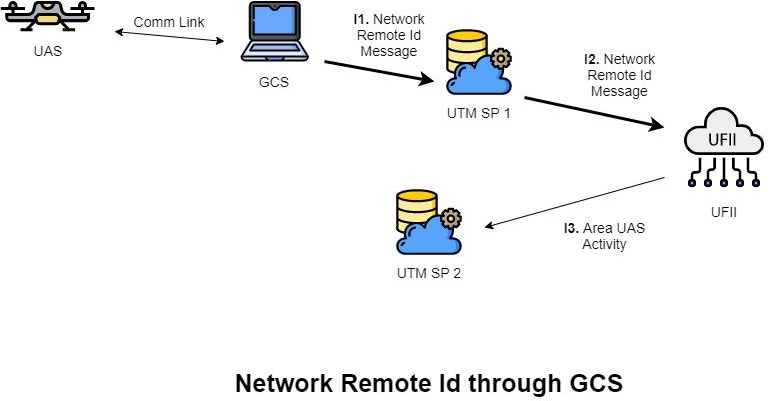
\includegraphics[height=0.2\textheight]{../images/nrid-uc01}
\par\end{centering}
}~\subfloat[NRID-UC02\label{nrid-uc02}]{\begin{centering}
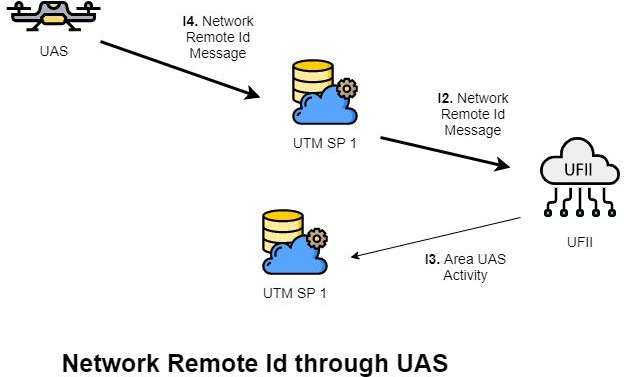
\includegraphics[height=0.2\textheight]{../images/nrid-uc02}
\par\end{centering}
}\\
\subfloat[No Remote ID (NORID-UC01)\label{norid-uc01}]{\centering{}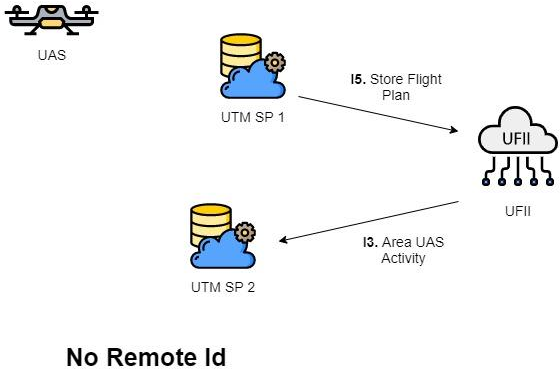
\includegraphics[height=0.2\textheight]{../images/norid-uc01}}
\par\end{centering}
\caption{Network Remote ID Use cases}

\end{figure}


\subsubsection{List of Interfaces}

See figures \ref{nrid-uc01}, \ref{nrid-uc02}, \ref{norid-uc01},
\ref{fig:BRID-UC01}.

\paragraph{Interface 1}

Send Remote Id Message (GCS -> UTM SP) 

\paragraph{Interface 2}

Send Remote Id Message (UTM SP -> UFII) 

\paragraph{Interface 3}

Area UAS Activity (UFII -> UTM SP) 

\paragraph{Interface 4}

Send Remote Id Message (UAS -> UFII) 

\paragraph{Interface 5}

Store Flight Plan (UTM SP -> UFII)


\subsubsection{Non-equipped UAS}

UAS that do not adhere to the Digital Sky framework are outside the
information system available. The most common scenario of identifying
a UAS flying overhead can be done using Digital Sky without any modification
to an NPNT compliant UAS, as every flight is notified before takeoff
and Digital sky can provide information on flights happening overhead
which have been planned. Flights outside of the Digital Sky Ecosystem
(illegal ones according to the UAS regulations) will fail to be identified
this way. Such drones will require a more complete Remote ID solution
and their compliance to any future remote ID regulations is a policy
enforcement issue. 

It should however be noted that when considering BVLOS operations,
broadcast remote ID will play a more important role in aiding deconfliction,
and is essential for operating in remote Areas where Network Remote
ID is not available. 


\subsection{Open Questions}

\subsubsection{Messaging proposals}

\paragraph{Forwarding}

UFII \&/or DigitalSky should provide an available endpoint for any
and all messaging, including Remote ID (Network) messages. These would
be forwarded to the relevant UTM-SP.

\paragraph{DSS + P2P}

UFII and/or DigitalSky should provide a Discovery and Synchronisation
Service that allows Operators/Pilots/UASs to discover UTM-SPs in the
region of operation and their messaging API endpoints. Following ``Discovery''
and choice of UTM-SP is made, messages are directed to that UTM-SP's
API endpoints.

\subsubsection{General availability of Telemetry\label{subsec:availability-Telemetry}}

Use-case: 

\[
\text{General Public}\ensuremath{\xrightarrow{\text{query UAS/Network RId+telemetry}}}\text{UTM SP}
\]
 

Member of the general public should be able to view/query Telemtery
data of UASs in area; typical application: view on map.
\begin{enumerate}
\item no
\item restrict to 50m radius around actor
\item no restrictions
\end{enumerate}

\subsubsection{General availability of Operational Authorisation or Data\label{subsec:availability-of-operational}}

Is the use-case: 

\[
\text{General Public}\ensuremath{\xrightarrow{\text{query UAS/Operation Data or Authorisation by Network RId}}}\text{UTM SP}
\]
 

one which must be addressed immediately, or when public demand for
it is apparent?

Options: 
\begin{enumerate}
\item no
\item 50m
\item restrict
\end{enumerate}

\subsubsection{Case by case}

For each use case figures \ref{nrid-uc01}, \ref{nrid-uc02}, \ref{norid-uc01},
\ref{fig:BRID-UC01}
\begin{enumerate}
\item What should be the interaction flow?
\item Request-Response or Publish-Subscribe?
\item What messaging protocol to use?
\begin{enumerate}
\item Possible options: MQTT, XMPP
\end{enumerate}
\item What network layer protocol to use?
\begin{enumerate}
\item Possible options: TCP/IP, UDP
\end{enumerate}
\item What should be the data format?
\begin{enumerate}
\item Possible options: JSON, XML, Thrift, Protobuf
\end{enumerate}
\item What data should be signed and how?
\item What data should be encrypted and how? 
\item Single/Multi UTM-SP in same operational volume
\begin{enumerate}
\item Which uses cases have any ramifications
\end{enumerate}
\end{enumerate}

\subsubsection{Remote ID Data}
\begin{enumerate}
\item By default, all fields as listed in Table 1 of ASTM Remote Id Spec
can be public. Possible exceptions could be Operator Position and
Identity. Need to come up with an encryption mechanism to transmit
sensitive data which should only be accessible to authorized entities. 
\begin{enumerate}
\item Encryption or omission?
\item If encryption, who is the intended recipient?
\end{enumerate}
\end{enumerate}


\paragraph{Hardware}
\begin{itemize}
\item A built-in or add-on hardware device that regularly sends a set of
flight parameters, including but not limited to a drone\textquoteright s
location, barometric altitude, the drone\textquoteright s serial number
(ANSI/CTA-2063 Physical Serial Number format) and the operator registration
ID over a wireless network to a tracking data collector.
\item The tracking data collector is a dedicated server that processes and
optionally stores the flight data. These data are forwarded to applications
that subscribe to the flight data, such as UTM systems.
\item Facilitating regulation which would require all UAS (or all UAS fulfilling
a certain set of criteria) to be mandatorily fitted with a (built-in
or add-on) Network Remote ID transmitting device and regulations requiring
the device to be actually transmitting. In the United States, the
FAA in its draft Regulation has proposed that virtually all UAS should
be covered, which perhaps goes too far. A
\item Facilitating regulation which would govern the activities of the location
data collector service providers (DCSP). Such regulation would need
to cover, e.g., what data the DCSP would supply to DSSPs (e.g. for
tactical deconfliction), what data would be supplied to the UFII /
Digital Sky, etc. Such regulation would also need to take into consideration
possible business models which would enable the smooth running of
the Network Remote ID / Tracking infrastructure. 
\end{itemize}


\subsection{Broadcast ID}

The broadcast protocol can be adopted as is from the ASTM standard

\begin{figure}[tbh]
\begin{centering}
\subfloat[BRID-UC01\label{fig:BRID-UC01}]{\begin{centering}
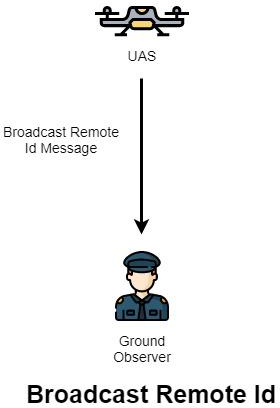
\includegraphics[height=0.2\textheight]{../images/brid-uc01}
\par\end{centering}
}
\par\end{centering}
\caption{Broadcast Remote ID Use cases}
\end{figure}


\section{Hardware}

\subsection{Security aspects: Programmability}
\begin{enumerate}
\item Who should be able to program the remote ID into hardware: Manufacturer/Operator/Pilot?
\item Is it One-Time-Programmable? If not how do we secure reprogramming
process?
\item What if it is an add-on hw module?
\item What if it is part of UAS Model?
\item Perhaps the programmer should have an auditable process
\item Is it possible to have a cryptographically secure process for this
similar to NPNT?
\end{enumerate}

\section{Adoption}
\begin{enumerate}
\item How would existing drones without any compliant RemoteID hardware
become compliant?
\begin{enumerate}
\item Integrating with Remote ID hardware on market (to be imported, integrated
and tested)
\item development of Remote ID chip/board in-house (open-sourced designs\footnote{Needs citation}
are available) \& integration
\end{enumerate}
\item What should the timeline be? Survey of business cases \& timelines
by stakeholder
\begin{enumerate}
\item 9 months
\begin{enumerate}
\item 6 months: product development/integration, testing
\item 3 months compliance testing \& approval
\item Leeway: 3 months
\end{enumerate}
\item UFII-UTM infrastructure for enablement
\begin{enumerate}
\item Development of protocols (2 months)
\item implementation (6 months)
\end{enumerate}
\item Operators \& Pilots
\begin{enumerate}
\item Training (?? months)
\end{enumerate}
\item Law Enforcement
\begin{enumerate}
\item Additional Hardware (?? months)
\item UTM-SP/UFII integration (?? months)
\item Training (3 months - 2 years)
\end{enumerate}
\end{enumerate}
\item Level of requirements\footnote{Use https://www.ietf.org/rfc/rfc2119.txt}
by use case
\item and cost to stakeholders, primarily Manufacturers
\begin{enumerate}
\item Compliances \& Import costs
\end{enumerate}
\end{enumerate}

\section{Conclusions and Future work}

We have outlined the ways in which Remote ID could by realistically
adopted in India. Unless there are strong reasons to deviate, the
ASTM standard should be adopted in India. While this chapter details
the technical standardisation effort to date, specific recommendations
for future policy making and regulation for unmanned aviation are
noted in the following chapter.

\cleardoublepage{}

\chapter{Recommendations}

\section{Regulation}

TBD

\section{Policy making}

TBD

\cleardoublepage{}

\chapter{Appendix}

\section{Pending changes}
\begin{enumerate}
\item Rakesh's editorial comments
\item Avianco's input on Network Remote ID use cases
\item Section on Security: spoofing and attacks
\item Review sections \ref{subsec:availability-Telemetry}, \ref{subsec:availability-of-operational}
from ASTM spec
\end{enumerate}

\section{General notes}


\paragraph{Possibility of provision of Remote ID for non-NPNT compliant drones.}

It is strongly recommended that the concepts of compliance and identification
should be separately tracked. A comparison would be: a car on the
road must have always a licence plate (identity); if it does not pass
a pollution control, or has faulty brakes, it is not compliant to
traffic rules. Broadcast, and in particular Network Remote ID is inclusive
rather than exclusive. 


\paragraph{Supplementary benefits of Remote ID}
\begin{itemize}
\item Increase UAS remote pilot accountability by removing anonymity
\item Data security. If required, the tracking information could be kept
entirely within the implementing country (cf tracking via GCS, where
there is no easy method of knowing where the information resides abroad).
\end{itemize}


\subsection{Serial Number format ANSI/CTA-2063-A\label{subsec:ANSI-CTA-2063-A}}

A Serial number \texttt{MFR1C123456789ABC} may be interpreted as 
\begin{description}
\item [{Manufacturer~Code}] \texttt{MFR1}, first 4 characters
\item [{Length~Code}] \texttt{C}, signifying the following 12 characters
are the unit serial number
\item [{Unit~Serial~Number}] \texttt{123456789ABC}
\end{description}

\section{Operational Scenarios}

\begin{table}[tbh]
\begin{centering}
\begin{tabular}{|c|c|c|c|}
\hline 
\textbf{\#} & \textbf{Cf.} &  & \tabularnewline
\hline 
\hline 
S01 & SORA/STS01 & VLoS & \tabularnewline
\hline 
S02 & SORA/STS02 & BVLoS & \tabularnewline
\hline 
S03 & FAA/V2-1 & Nominal UTM Operations in Uncontrolled and Controlled Airspace & \tabularnewline
\hline 
S04 & FAA/V2-2 & UVRs and Associated Operational Impacts & \tabularnewline
\hline 
S05 & FAA/V2-3 & Interactions between UAS and Manned Aircraft at Low Altitudes & \tabularnewline
\hline 
S06 & FAA/V2-4 & Use of UTM to Remotely Identify UAS & \tabularnewline
\hline 
S07 & FAA/V2-5 & Federal Public Safety Request for UTM Information & \tabularnewline
\hline 
 & EASA/STS-01 &  & $\equiv$S01\tabularnewline
\hline 
 & EASA/STS-02 &  & $\equiv$S02\tabularnewline
\hline 
\end{tabular}
\par\end{centering}
\caption{Operational Scenarios}

\end{table}


\section{Operational Use cases}

\begin{table}[tbh]
\begin{centering}
\begin{tabular}{|l|l|}
\hline 
\textbf{\#} & \textbf{Description}\tabularnewline
\hline 
\hline 
TCL1-1 & Two VLOS Operations with Voluntary Use of UTM for Coordination\tabularnewline
\hline 
TCL2-1 & One BVLOS Operation, One VLOS Operation with Voluntary UTM Participation
for Coordination\tabularnewline
\hline 
TCL2-2 & Two BVLOS Operations near an Airport in Uncontrolled Airspace\tabularnewline
\hline 
TCL2-3 & Priority Operation \textendash{} Emergency Medical Aircraft in Uncontrolled
Airspace\tabularnewline
\hline 
TCL2-4 & BVLOS Operation Conformance Violation from Uncontrolled Airspace into
Class D Airspace\tabularnewline
\hline 
TCL3-1 & One-Way BVLOS Flight, Separate Landing/Take-Off Locations\tabularnewline
\hline 
TCL3-2 & Negotiation versus Prioritization between Operators Due to Dynamic
Restriction\tabularnewline
\hline 
TCL3-3 & UAS Interaction with Manned Aircraft in Low-Altitude Uncontrolled
Airspace\tabularnewline
\hline 
TCL3-4 & BVLOS Operation Lost-Link Event\tabularnewline
\hline 
TCL3-5 & High Density UTM Operations in Uncontrolled Airspace\tabularnewline
\hline 
TCL3-6 & Last-Mile Rural Deliveries in Uncontrolled Airspace under the Mode
C Veil\tabularnewline
\hline 
TCL3-7 & UAS Operator Loss of Performance Capabilities in Uncontrolled Airspace\tabularnewline
\hline 
TCL4-1 & BVLOS UTM Operation within UAS Facility Maps\tabularnewline
\hline 
TCL4-2 & Historical UTM Information Queries by Authorized Entities\tabularnewline
\hline 
TCL4-3 & UAS Urgency/Distress Condition with Alternate Landing and UTM Coordination\tabularnewline
\hline 
TCL4-4 & UAS Volume Reservation in Controlled Airspace\tabularnewline
\hline 
TCL4-5 & Report to FAA due to UAS Flight Incident\tabularnewline
\hline 
 & Night-time VLoS/BVLoS\tabularnewline
\hline 
\end{tabular}
\par\end{centering}
\caption{}

\end{table}


\section{Scenario/use-case wise data compliance requirements}

\begin{table}[tbh]
\begin{centering}
\begin{tabular}{|c|c|c|c|c|c|c|}
\hline 
Scenario & Cf. & Broadcast &  & Network &  & \tabularnewline
\hline 
\hline 
VLoS & SORA/STS01 & $\CIRCLE$ $\LEFTcircle$ $\varodot$ $\varobslash$ $\varotimes$ &  & $\CIRCLE$ $\LEFTcircle$ $\varodot$ $\varobslash$ $\varotimes$ &  & \tabularnewline
\hline 
BVLoS & SORA/STS02 & $\CIRCLE$ $\LEFTcircle$ $\varodot$ $\varobslash$ $\varotimes$ &  & $\CIRCLE$ $\LEFTcircle$ $\varodot$ $\varobslash$ $\varotimes$ &  & \tabularnewline
\hline 
 &  & $\CIRCLE$ $\LEFTcircle$ $\varodot$ $\varobslash$ $\varotimes$ &  & $\CIRCLE$ $\LEFTcircle$ $\varodot$ $\varobslash$ $\varotimes$ &  & \tabularnewline
\hline 
 &  & $\CIRCLE$ $\LEFTcircle$ $\varodot$ $\varobslash$ $\varotimes$ &  & $\CIRCLE$ $\LEFTcircle$ $\varodot$ $\varobslash$ $\varotimes$ &  & \tabularnewline
\hline 
 &  & $\CIRCLE$ $\LEFTcircle$ $\varodot$ $\varobslash$ $\varotimes$ &  & $\CIRCLE$ $\LEFTcircle$ $\varodot$ $\varobslash$ $\varotimes$ &  & \tabularnewline
\hline 
 &  & $\CIRCLE$ $\LEFTcircle$ $\varodot$ $\varobslash$ $\varotimes$ &  & $\CIRCLE$ $\LEFTcircle$ $\varodot$ $\varobslash$ $\varotimes$ &  & \tabularnewline
\hline 
\end{tabular}
\par\end{centering}
\begin{centering}
\begin{lyxgreyedout}
\begin{center}
{*}not a great idea
\par\end{center}%
\end{lyxgreyedout}
\par\end{centering}
\caption{Operational Scenario vs Compliance requirements: $\CIRCLE$ Mandatory,
$\protect\LEFTcircle$Recommended, $\varodot$ Optional, $\varobslash$
Not Recommended, $\varotimes$ Forbidden}
\end{table}


\section{Supplementary Comments}

\subsection{Lifetime\label{subsec:Lifetime}}

Technically, there is no need for UIN to change during the lifetime
of a drone. Questions arise as to
\begin{enumerate}
\item how should \textquotedblleft lifetime\textquotedblright{} be defined:
options for basis
\begin{enumerate}
\item flight controller board or PKI/X.509
\begin{enumerate}
\item multiple PKI/X.509 per UAS 
\item replacement of PKI/X.509 in case of key compromise
\end{enumerate}
\item Manufacturer Serial no (akin to chassis no.)
\item Physical unclonable function\footnote{Not currently realistic} (PUF)
or alternatives
\end{enumerate}
\item how should component changes by manufacturer or owner be treated
\begin{enumerate}
\item should scheduled maintenance/parts replacement be reported to UFII?
\end{enumerate}
\end{enumerate}

\paragraph{Hobbyist and research sector}

\begin{lyxgreyedout}
summarise applicability, etc. FAA NPRM Public page notes 54K comments
from the general public; concerns raised include stifling innovation
and the hobbyist sectors because of increased compliance requirements
for no added security (which is not strictly true). These sectors
should be allowed certain leeway in compliance, at the same time be
made aware of liability concerns in case of mishaps. %
\end{lyxgreyedout}


\section*{Acknowlegment}

\begin{lyxgreyedout}
TODO

@cf Altitude Angel, https://auterion.com/skynode/%
\end{lyxgreyedout}

\bibliographystyle{IEEEtran}
\bibliography{../Bibliography}

\end{document}
